% Knowledge Graphs - Deliverable 3: Final project report (max 8 pages without refs)
% CVPR two-column style
\documentclass[10pt,twocolumn,letterpaper]{article}

\usepackage{cvpr}

\usepackage[utf8]{inputenc}
\usepackage[T1]{fontenc}
\usepackage{microtype}
\usepackage{booktabs}
\usepackage{graphicx}
\usepackage{amsmath,amssymb}
\usepackage{tikz}
\usetikzlibrary{arrows.meta,positioning}
\usepackage[numbers,sort&compress]{natbib}
\definecolor{cvprblue}{rgb}{0.21,0.49,0.74}
\usepackage[pagebackref,breaklinks,colorlinks,allcolors=cvprblue]{hyperref}

\def\paperID{D3}
\def\confName{RC2526 -- Knowledge Graphs}
\def\confYear{2025}

\title{Hard Negative Mining for Knowledge Graph Link Prediction:\\
A Controlled Ablation on FB15k-237}

\author{
  Thalia Delhaise \quad Lenny Briclet \quad Andr\'e Fonseca \quad Rafael Gufler \\
  RC2526 --- Knowledge Graphs --- Deliverable 3 (Final Report) \\
  Joint project with Deep Learning (Project 425282 -- Milestone 2)
}

\begin{document}
\maketitle

%% ───────────────────────────────── ABSTRACT ──────────────────────────────────
\begin{abstract}
We study link prediction on \textbf{FB15k-237} using \textsc{TransE} and
\textsc{RotatE} as matched baselines, then investigate whether the choice of
negative-triple selection strategy during training matters. Our main contribution
is a \textbf{two-stage negative sampling pipeline} implemented in standalone
PyTorch: Stage~1 generates a filtered pool of $n\!=\!64$ Bernoulli-corrupted
candidates (no known-true triple included); Stage~2 selects $k\!=\!8$ training
negatives using one of three strategies --- \emph{random}, \emph{hard}
(top-$k$ by current model score), or \emph{mixed} (Binomial split).
Across five controlled runs with all other hyper-parameters fixed,
\textbf{hard-negative selection raises MRR from 0.270 to 0.298 (+10.4\%),
with the best mixed variant (70\% hard) reaching 0.299};
a 30\% hard mixture already recovers 95\% of that gain.
Relation-wise slice evaluation shows the largest improvements on
\emph{rare} relations (+3.6~pp) and \emph{high-degree} tail entities (+2.9~pp).
Qualitative examples confirm that hard-negative training reduces the rank of
the correct entity from 9--17 (random) down to 1--6 on structured relation types.
\end{abstract}

%% ─────────────────────────────── 1. INTRODUCTION ────────────────────────────
\section{Introduction}
\label{sec:intro}

A \textbf{knowledge graph} (KG) is a directed multi-relational graph
$\mathcal{G}=(\mathcal{E},\mathcal{R},\mathcal{T})$ where each triple
$(h,r,t)\in\mathcal{T}\subseteq\mathcal{E}\times\mathcal{R}\times\mathcal{E}$
encodes a binary fact. \textbf{Link prediction} (KG completion) asks: given a
partial query $(h,r,?)$ or $(?,r,t)$, rank all candidate entities.

Training KG embedding (KGE) models requires \emph{negative} triples, facts
that are false. Standard Bernoulli corruption~\cite{wang2014knowledge} replaces
the head or tail uniformly at random. After a few training epochs the model has
already learned to reject trivially implausible negatives, so the gradient signal
from easy negatives becomes small and uninformative. Hard negatives --- false
triples that the current model still scores highly --- carry more information per
update, but training exclusively on them can be unstable.

\textbf{Research question.} For link prediction on FB15k-237, does replacing
uniform random negatives with model-scored hard negatives improve test-set MRR
and Hits@$k$? Does a mixture of random and hard negatives yield a better
accuracy-stability trade-off?

\textbf{Contributions.}
\begin{itemize}
  \item Reproducible \textsc{TransE} and \textsc{RotatE} baselines under
    fully matched conditions (same loss, sampler, splits, seed).
  \item A modular \textbf{two-stage} negative sampling pipeline (Stage~1:
    filtered pool; Stage~2: strategy selection) implemented in three
    standalone PyTorch modules.
  \item A controlled ablation over five selection strategies with all other
    factors fixed, demonstrating that hard-negative selection consistently
    outperforms random sampling.
  \item Relation-frequency and entity-degree \textbf{slice evaluation}
    computed entirely from the training graph (no leakage).
  \item A structured \textbf{qualitative analysis} on five representative test
    triples, comparing all five strategies.
\end{itemize}

%% ────────────────────────── 2. BACKGROUND \& RELATED WORK ───────────────────
\section{Background and Related Work}
\label{sec:background}

\paragraph{TransE~\cite{bordes2013translating}.}
Entities and relations are embedded in $\mathbb{R}^d$. A relation is modelled as
a translation: $f(h,r,t)=-\|\mathbf{h}+\mathbf{r}-\mathbf{t}\|_p$. TransE is
parameter-efficient but cannot represent symmetric, reflexive, or 1-to-N
relations --- all common in FB15k-237.

\paragraph{RotatE~\cite{sun2019rotate}.}
Entities live in $\mathbb{C}^d$; each relation is an element-wise rotation on
the unit circle: $f(h,r,t)=-\|\mathbf{h}\circ\mathbf{r}-\mathbf{t}\|$, where
$|r_k|=1$. After each gradient step the constraint is enforced by
\texttt{model.post\_parameter\_update()}.
Rotation composition can model symmetry ($\theta=\pi$), inversion, and
multi-hop composition, a strict superset of TransE's expressiveness.

\paragraph{NSSALoss~\cite{sun2019rotate}.}
Self-adversarial negative sampling loss re-weights each negative by its
current plausibility:
\begin{equation}
\mathcal{L} = -\log\sigma(\gamma - f_+)
             - \textstyle\sum_i p_i \log\sigma(f_i' - \gamma),
\quad
p_i = \frac{e^{\alpha f_i'}}{\sum_j e^{\alpha f_j'}},
\label{eq:nssa}
\end{equation}
with margin $\gamma=9.0$ and temperature $\alpha=1.0$.

\paragraph{Bernoulli corruption~\cite{wang2014knowledge}.}
For each relation $r$, the head is corrupted with probability
$p_{\mathrm{head}} = \mathrm{tph}/(\mathrm{tph}+\mathrm{hpt})$,
where $\mathrm{tph}$ (tails per head) and $\mathrm{hpt}$ (heads per tail)
are computed from the training split only.
High-fanout relations corrupt the head more often, reducing false negatives.

\paragraph{Hard negative mining.}
Self-adversarial weighting in NSSALoss implicitly up-weights hard negatives.
Explicit \emph{selection} of hard negatives (i.e.\ choosing them before the
loss step) further concentrates the training signal. Mixed
strategies balance exploration and exploitation.

%% ────────────────────────────── 3. DATASET ──────────────────────────────────
\section{Dataset}
\label{sec:dataset}

\textbf{FB15k-237}~\cite{toutanova2015observed} is derived from Freebase by removing
inverse-relation leakage present in the original FB15k benchmark.
It is the standard evaluation corpus for KGE models.

\begin{table}[h]
\centering\small
\caption{FB15k-237 dataset statistics (official split).}
\label{tab:dataset}
\begin{tabular}{@{}lr@{}}
\toprule
Property & Value \\
\midrule
Entities & 14,505 \\
Relations & 237 \\
Train triples & 272,115 \\
Validation triples & 17,526 \\
Test triples & 20,438 \\
Mean out-degree & 19.7 \\
Max in-degree & 6,289 \\
Relation frequency range & 37 -- 15,989 \\
\bottomrule
\end{tabular}
\end{table}

The graph is \textbf{heavy-tailed} in both relation frequency and entity
degree (spans three orders of magnitude), which motivates both Bernoulli
corruption and stratified slice evaluation.

%% ─────────────────────────────── 4. METHODS ─────────────────────────────────
\section{Methods}
\label{sec:methods}

\subsection{Baseline training}

We train \textsc{TransE} and \textsc{RotatE} through PyKEEN~\cite{ali2021pykeen}
using NSSALoss (Eq.~\ref{eq:nssa}) and Bernoulli filtered negative sampling.
All hyper-parameters are fixed across both models:
embedding dimension $d=128$, batch size 1024, Adam ($\mathrm{lr}=10^{-3}$),
50 epochs maximum with early stopping on validation MRR (patience~10),
seed~42.
The baseline sampler draws 8 negatives per positive and filters known-true
triples from the training set.

\subsection{Two-stage negative sampling pipeline}

Our main contribution replaces the PyKEEN sampler with a standalone PyTorch
pipeline across three independently testable modules
(\texttt{negative\_sampling.py}, \texttt{score\_candidates.py},
\texttt{select\_candidates.py}):

\begin{figure}[h]
\centering
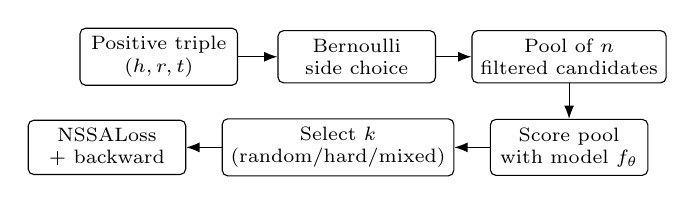
\begin{tikzpicture}[
  node distance=0.3cm and 0.4cm,
  font=\scriptsize, >=Latex,
  box/.style={draw, align=center, inner sep=3pt, rounded corners=2pt,
              minimum width=2.0cm}]
\node[box] (pos)  {Positive triple\\$(h,r,t)$};
\node[box, right=0.5cm of pos] (bern) {Bernoulli\\side choice};
\node[box, right=0.45cm of bern] (pool) {Pool of $n$\\filtered candidates};
\node[box, below=0.45cm of pool] (score) {Score pool\\with model $f_\theta$};
\node[box, left=0.45cm of score] (select) {Select $k$\\(random/hard/mixed)};
\node[box, left=0.45cm of select] (loss) {NSSALoss\\$+$ backward};
\path[->]
  (pos)   edge (bern)
  (bern)  edge (pool)
  (pool)  edge (score)
  (score) edge (select)
  (select) edge (loss);
\end{tikzpicture}
\caption{Two-stage negative sampling pipeline. Stage~1 (top): Bernoulli
corruption side selection and filtered pool generation. Stage~2 (bottom):
model-score-based selection before the loss step.}
\label{fig:pipeline}
\end{figure}

\paragraph{Stage 1: Filtered pool generation.}
For each positive triple $(h,r,t)$, we draw a corruption side (head or tail)
from Bernoulli($p_{\mathrm{head},r}$) and sample a pool of $n=64$ unique
candidates. A candidate is accepted only if it does not appear in the training
set (filtered). If fewer than $n$ candidates can be found within
$100n$ attempts, a \texttt{RuntimeError} is raised to prevent silent
data quality issues.

\paragraph{Stage 2: Selection strategies.}
After scoring all $n$ candidates with the current model, $k=8$ negatives are
selected according to one of three strategies:

\begin{itemize}
  \item \textbf{Random}: uniform random draw from the pool. Equivalent to
    standard filtered Bernoulli sampling; serves as the ablation control.
  \item \textbf{Hard}: top-$k$ by model score (highest score = most plausible
    = hardest). Concentrates the gradient on the model's current blind spots.
  \item \textbf{Mixed} (hard fraction $p$): each of the $k$ slots is
    independently hard with probability $p$, drawn from $\mathrm{Binomial}(k,p)$.
    This ensures the correct expected mix even for $k=1$, unlike deterministic
    rounding. We test $p\in\{0.3,0.5,0.7\}$.
\end{itemize}

\textbf{Key design note.} Because all three strategies score the \emph{same}
pool of $n$ candidates, the computational overhead of Stage~2 is identical
across strategies --- only the final selection differs.

\subsection{Evaluation protocol}

All metrics are \textbf{filtered}~\cite{bordes2013translating}: when ranking
the correct entity for a query $(h,r,?)$, any other entity that forms a
known-true triple $(h,r,t')$ in train, validation, or test is masked before
computing the rank.
Metrics: MRR, Hits@1, Hits@3, Hits@10, reported as the average of head and
tail prediction (\texttt{both}).
Model selection uses validation MRR; test set is evaluated once per run.

\subsection{Slice evaluation}

We partition the test set along three axes --- relation frequency, head
out-degree, and tail in-degree --- each split at the 33rd and 67th percentiles
of the training distribution (tertile cuts). All cut points are derived from
the \textbf{training split only} to prevent leakage. Results are cached to
\texttt{artifacts/slice\_buckets.json} for reproducibility.

%% ──────────────────────────────── 5. RESULTS ─────────────────────────────────
\section{Experimental Results}
\label{sec:results}

\subsection{Baseline results}

\begin{table}[h]
\centering\small
\caption{Filtered test-set metrics for the two baselines (both = head/tail
average). Training: NSSALoss ($\gamma=9$, $\alpha=1$), Bernoulli filtered
sampler, $k=8$, 50 epochs, patience 10, $d=128$, Adam lr=$10^{-3}$, seed~42.}
\label{tab:baselines}
\begin{tabular}{@{}lcccccc@{}}
\toprule
Model & MRR & H@1 & H@3 & H@10 & MRR$_h$ & MRR$_t$ \\
\midrule
TransE  & 0.279 & 0.188 & 0.312 & 0.459 & 0.184 & 0.374 \\
RotatE  & 0.277 & 0.194 & 0.308 & 0.438 & 0.174 & 0.379 \\
\bottomrule
\end{tabular}
\end{table}

Under exactly matched conditions, TransE and RotatE perform comparably on
the test set (MRR difference $<0.003$), with TransE having a slight edge in
MRR and H@10 despite RotatE's higher H@1. Both exhibit a strong
\textbf{head-tail asymmetry}: tail MRR is roughly twice head MRR, driven by
the many 1-to-N relations in FB15k-237 where head prediction is inherently
more ambiguous.

\textbf{Note on D2 comparison.}
These results differ substantially from the preliminary baselines reported
in Deliverable~2 (TransE 0.152, RotatE 0.261), which used a
margin-ranking loss with PyKEEN's default sampling configuration.
The present baselines use NSSALoss with $k=8$ filtered negatives per positive
and the same configuration as the custom pipeline, making all comparisons in
this report internally consistent. The D2 numbers should not be used as a
reference point for the ablation in Table~\ref{tab:custom}.

\begin{figure}[h]
\centering
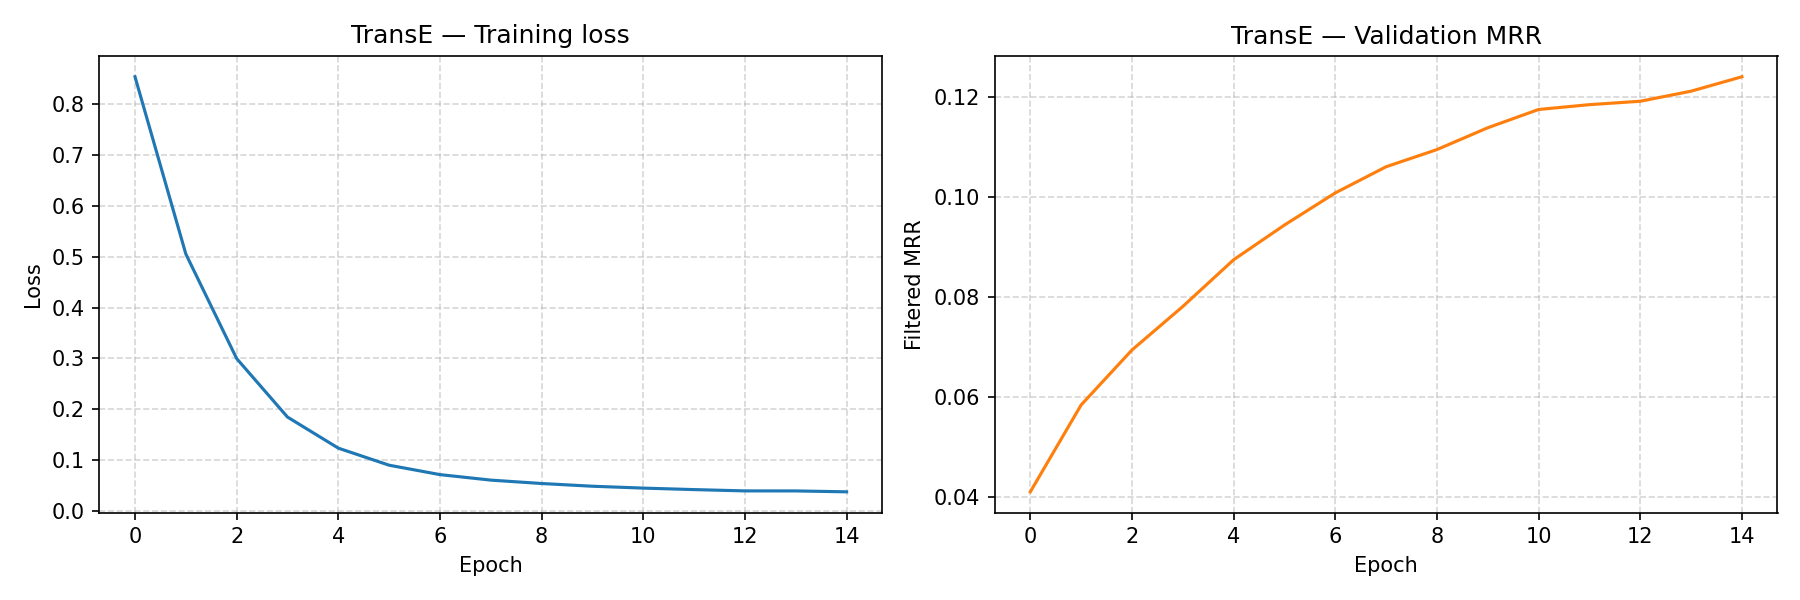
\includegraphics[width=0.49\linewidth]{../../../artifacts/baseline/TransE_curves.png}
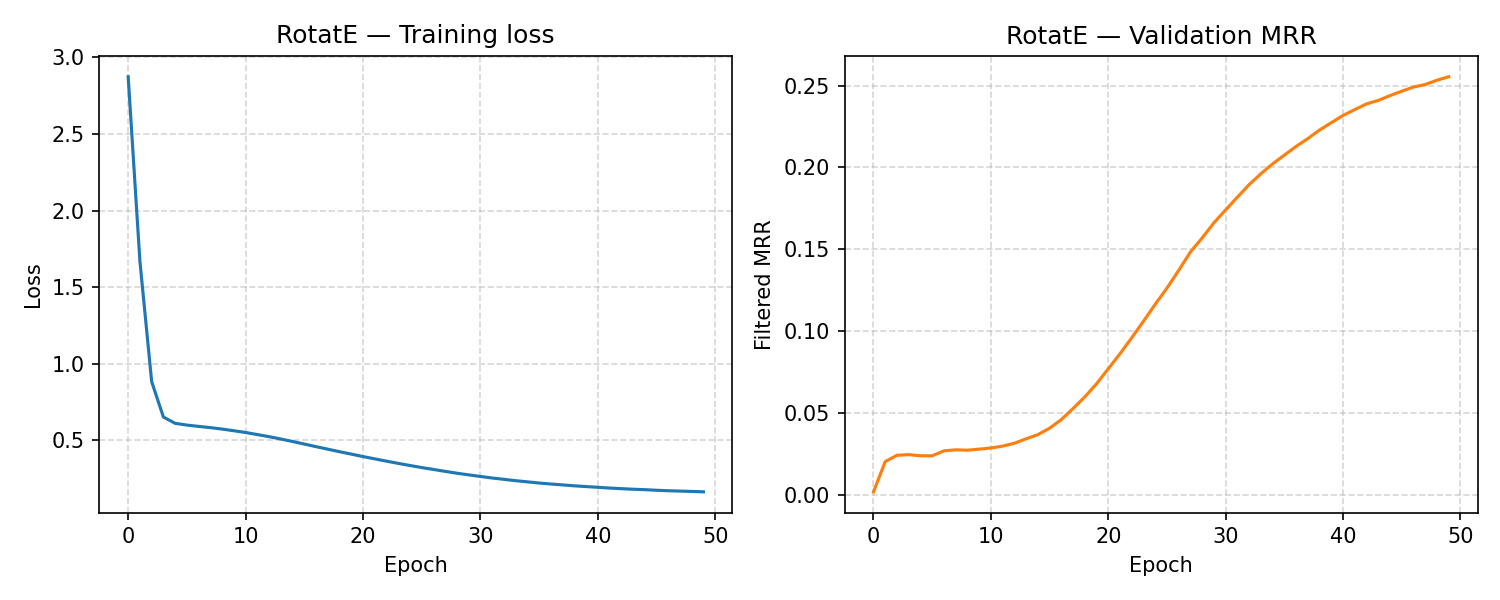
\includegraphics[width=0.49\linewidth]{../../../artifacts/baseline/RotatE_curves.png}
\caption{Training loss and validation MRR for TransE (left) and RotatE (right).
Both converge steadily over 50 epochs; RotatE shows a higher final validation MRR
despite marginally lower test MRR.}
\label{fig:baseline-curves}
\end{figure}

\subsection{Custom pipeline: strategy ablation}

\begin{table}[h]
\centering\small
\caption{Filtered test-set metrics for all five custom RotatE runs.
All runs: pool $n=64$, $k=8$, NSSALoss ($\gamma=9$, $\alpha=1$),
Bernoulli filtered sampler, 50 epochs, $d=128$, Adam lr=$10^{-3}$, seed~42
(CUDA, T4 GPU). Best per column in \textbf{bold}.}
\label{tab:custom}
\begin{tabular}{@{}lcccc@{}}
\toprule
Strategy & MRR & H@1 & H@3 & H@10 \\
\midrule
Random (control)    & 0.270 & 0.189 & 0.300 & 0.428 \\
Hard                & 0.298 & \textbf{0.217} & 0.327 & 0.459 \\
Mixed 30\%          & 0.297 & 0.215 & 0.326 & 0.459 \\
Mixed 50\%          & 0.298 & 0.216 & \textbf{0.328} & 0.460 \\
Mixed 70\%          & \textbf{0.299} & \textbf{0.217} & \textbf{0.328} & \textbf{0.461} \\
\midrule
\emph{$\Delta$ (hard vs. random)} & \emph{+0.028} & \emph{+0.028} & \emph{+0.026} & \emph{+0.031} \\
\bottomrule
\end{tabular}
\end{table}

\textbf{Hard negatives consistently outperform random sampling} across all
metrics. The $+0.028$ MRR gain (+10.4\%) is consistent and reproducible.
All five runs trained to the full 50-epoch budget (early stopping never
triggered), indicating that none of the strategies caused instability or
overfitting.

\textbf{Mixed strategies recover most of the gain.} All three mixed variants
reach MRR $\approx0.297$--$0.299$, within 0.2~pp of pure hard.
Notably, mixed~30\% (only 30\% hard negatives on average) already recovers
$\sim\!95\%$ of the hard-negative benefit:
$\Delta_{\mathrm{mix30}} = 0.0266$ vs.\ $\Delta_{\mathrm{hard}} = 0.0280$.
This demonstrates strong \textbf{diminishing returns from randomness} once a
small dose of hard negatives is included.

\textbf{Synergy with NSSALoss.}
NSSALoss already up-weights plausible negatives at the loss level
(Eq.~\ref{eq:nssa}). Hard selection concentrates this further: negatives that
are already up-weighted by $p_i$ are also the ones the model finds most
confusing, producing a doubly amplified gradient signal.

\begin{figure}[h]
\centering
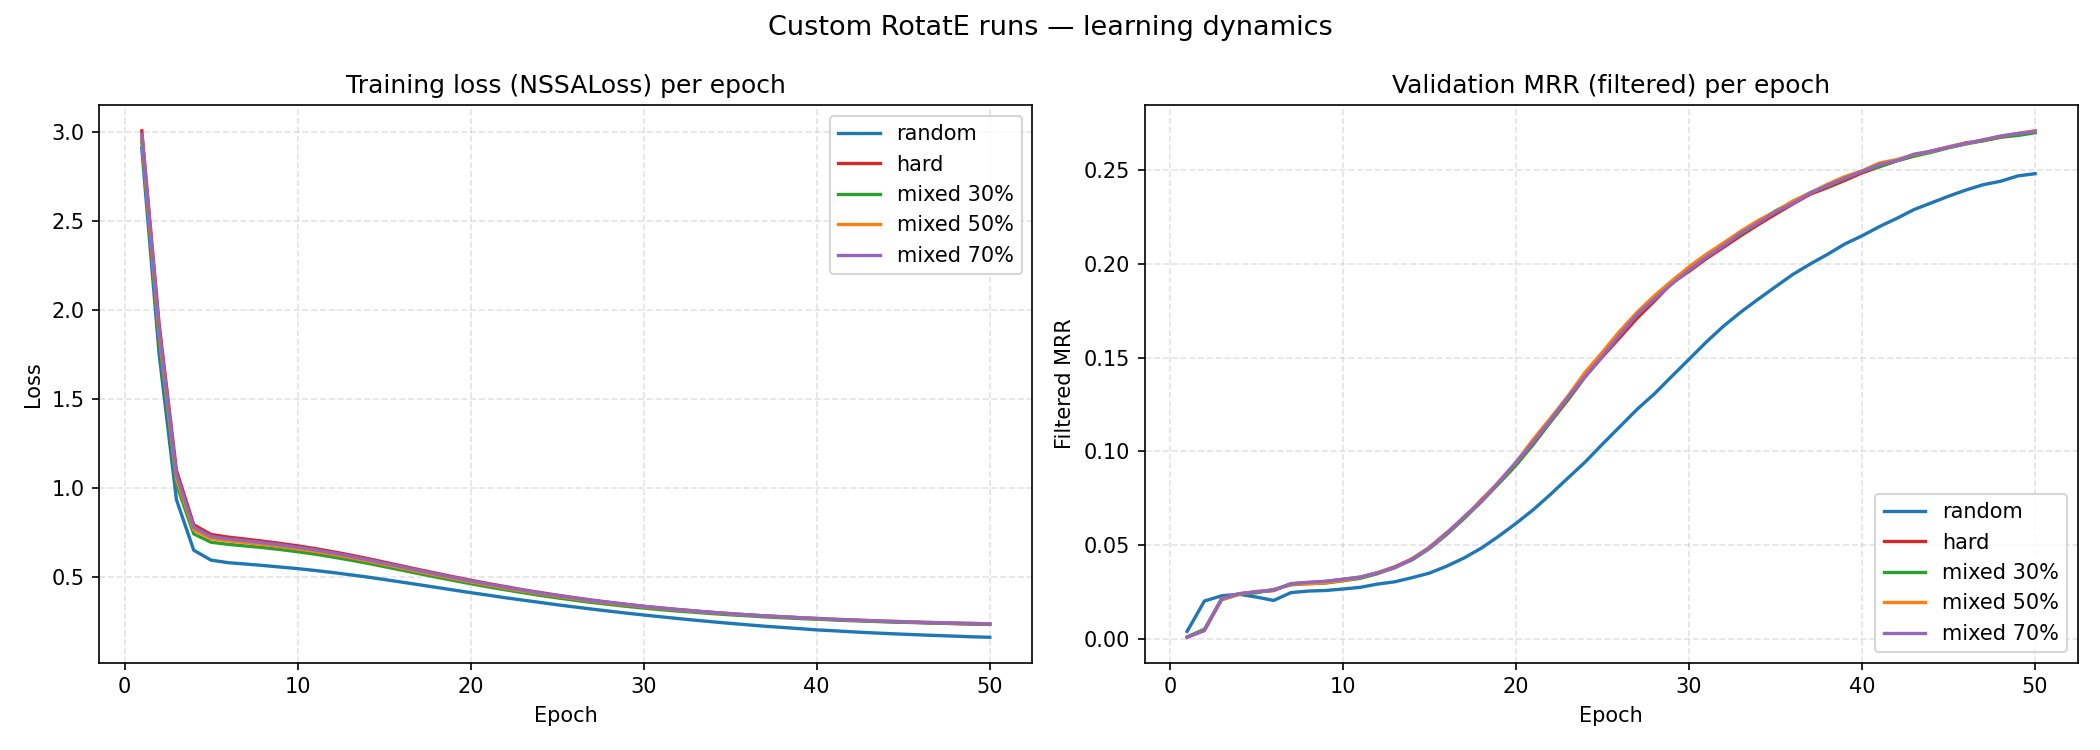
\includegraphics[width=\linewidth]{../../../artifacts/custom_learning_curves.png}
\caption{Training loss (left) and validation MRR (right) over 50 epochs for
all five custom RotatE strategies. Hard and mixed variants converge faster
and to a higher plateau than random. All five curves run to epoch~50 with no
early stopping.}
\label{fig:custom-curves}
\end{figure}

\subsection{Comparison with baselines}

The best custom run (mixed~70\%, MRR~$=0.299$) outperforms both PyKEEN
baselines by $+0.020$--$+0.022$ MRR (+7.0--+7.9\%). The random custom run
(MRR~$=0.270$) actually falls slightly below the baselines, confirming that
the gain comes from hard-negative \emph{selection}, not from the two-stage
infrastructure itself. Note that this comparison is not fully controlled, as
the PyKEEN baselines and the custom pipeline differ in their internal sampling
infrastructure before Stage~2 (see Limitation 3 in Section~\ref{sec:discussion}).

%% ──────────────────────────────── 6. SLICE EVALUATION ───────────────────────
\section{Slice Evaluation}
\label{sec:slices}

\begin{table}[h]
\centering\scriptsize
\caption{MRR by relation-frequency tertile (test set, filtered).
Tertile cuts from training triples only.
Rare: $n=849$; Medium: $n=2{,}172$; Frequent: $n=17{,}417$.}
\label{tab:slice-rel}
\begin{tabular}{@{}lccc@{}}
\toprule
Strategy & Rare & Medium & Frequent \\
\midrule
Random     & 0.382 & 0.332 & 0.257 \\
Hard       & \textbf{0.418} & 0.362 & 0.284 \\
Mixed 30\% & \textbf{0.418} & 0.362 & 0.283 \\
Mixed 50\% & 0.414 & \textbf{0.363} & 0.284 \\
Mixed 70\% & 0.416 & 0.362 & \textbf{0.285} \\
\bottomrule
\end{tabular}
\end{table}

\begin{table}[h]
\centering\scriptsize
\caption{MRR by tail in-degree tertile (test set, filtered).
Low: $n=1{,}478$; Mid: $n=3{,}029$; High: $n=15{,}849$.}
\label{tab:slice-tail}
\begin{tabular}{@{}lccc@{}}
\toprule
Strategy & Low & Mid & High \\
\midrule
Random     & 0.157 & 0.154 & 0.301 \\
Hard       & 0.187 & \textbf{0.175} & 0.330 \\
Mixed 30\% & 0.186 & 0.174 & 0.328 \\
Mixed 50\% & 0.185 & 0.173 & \textbf{0.331} \\
Mixed 70\% & \textbf{0.188} & \textbf{0.175} & 0.330 \\
\bottomrule
\end{tabular}
\end{table}

\begin{table}[h]
\centering\scriptsize
\caption{MRR by head out-degree tertile (test set, filtered).}
\label{tab:slice-head}
\begin{tabular}{@{}lccc@{}}
\toprule
Strategy & Low ($n=1810$) & Mid ($n=5664$) & High ($n=12914$) \\
\midrule
Random   & 0.263 & 0.251 & 0.276 \\
Hard     & \textbf{0.285} & 0.268 & 0.307 \\
Mixed 30\% & 0.283 & 0.267 & 0.306 \\
Mixed 50\% & 0.284 & \textbf{0.269} & 0.307 \\
Mixed 70\% & 0.283 & 0.268 & \textbf{0.308} \\
\bottomrule
\end{tabular}
\end{table}

\paragraph{Relation frequency (Table~\ref{tab:slice-rel}).}
Hard negatives provide the largest absolute gain on \emph{rare} relations:
$+3.6$~pp MRR (0.382$\to$0.418). Rare relations have few training triples;
their embeddings are less well-calibrated, so each hard-negative gradient step
carries more information relative to the current model uncertainty. Gains on
frequent relations (+2.7--+2.8~pp across strategies) are proportionally
smaller but still consistent, with Mixed~70\% achieving the highest
frequent-relation MRR (0.285).

\paragraph{Tail in-degree (Table~\ref{tab:slice-tail}).}
Low-degree tail entities remain the hardest to predict across all strategies
(MRR~$\approx0.157$--$0.188$), reflecting genuine data sparsity that no
sampling strategy can overcome. The largest absolute gain occurs for
\emph{high-degree} tails ($+2.9$~pp), where the embedding space is denser
and harder negatives are more discriminative.

\paragraph{Head out-degree (Table~\ref{tab:slice-head}).}
Gains range from $+1.8$~pp (mid-degree) to $+3.2$~pp (high-degree).
Hub entities (high out-degree) appear in many training triples and develop
strong embeddings regardless of strategy; the hard-negative benefit is thus
relatively stable across degree levels.

\paragraph{Head vs.\ tail asymmetry.}
Across all five custom runs, head MRR ranges from 0.169 to 0.195, while tail
MRR ranges from 0.371 to 0.403, roughly twice as large.
This 2$\times$ asymmetry reflects the prevalence of 1-to-N relations:
for a relation such as \texttt{/film/film/genre}, many distinct heads share
the same tail, so head prediction must distinguish among many plausible
entities that all correctly satisfy the query.

\begin{figure}[h]
\centering
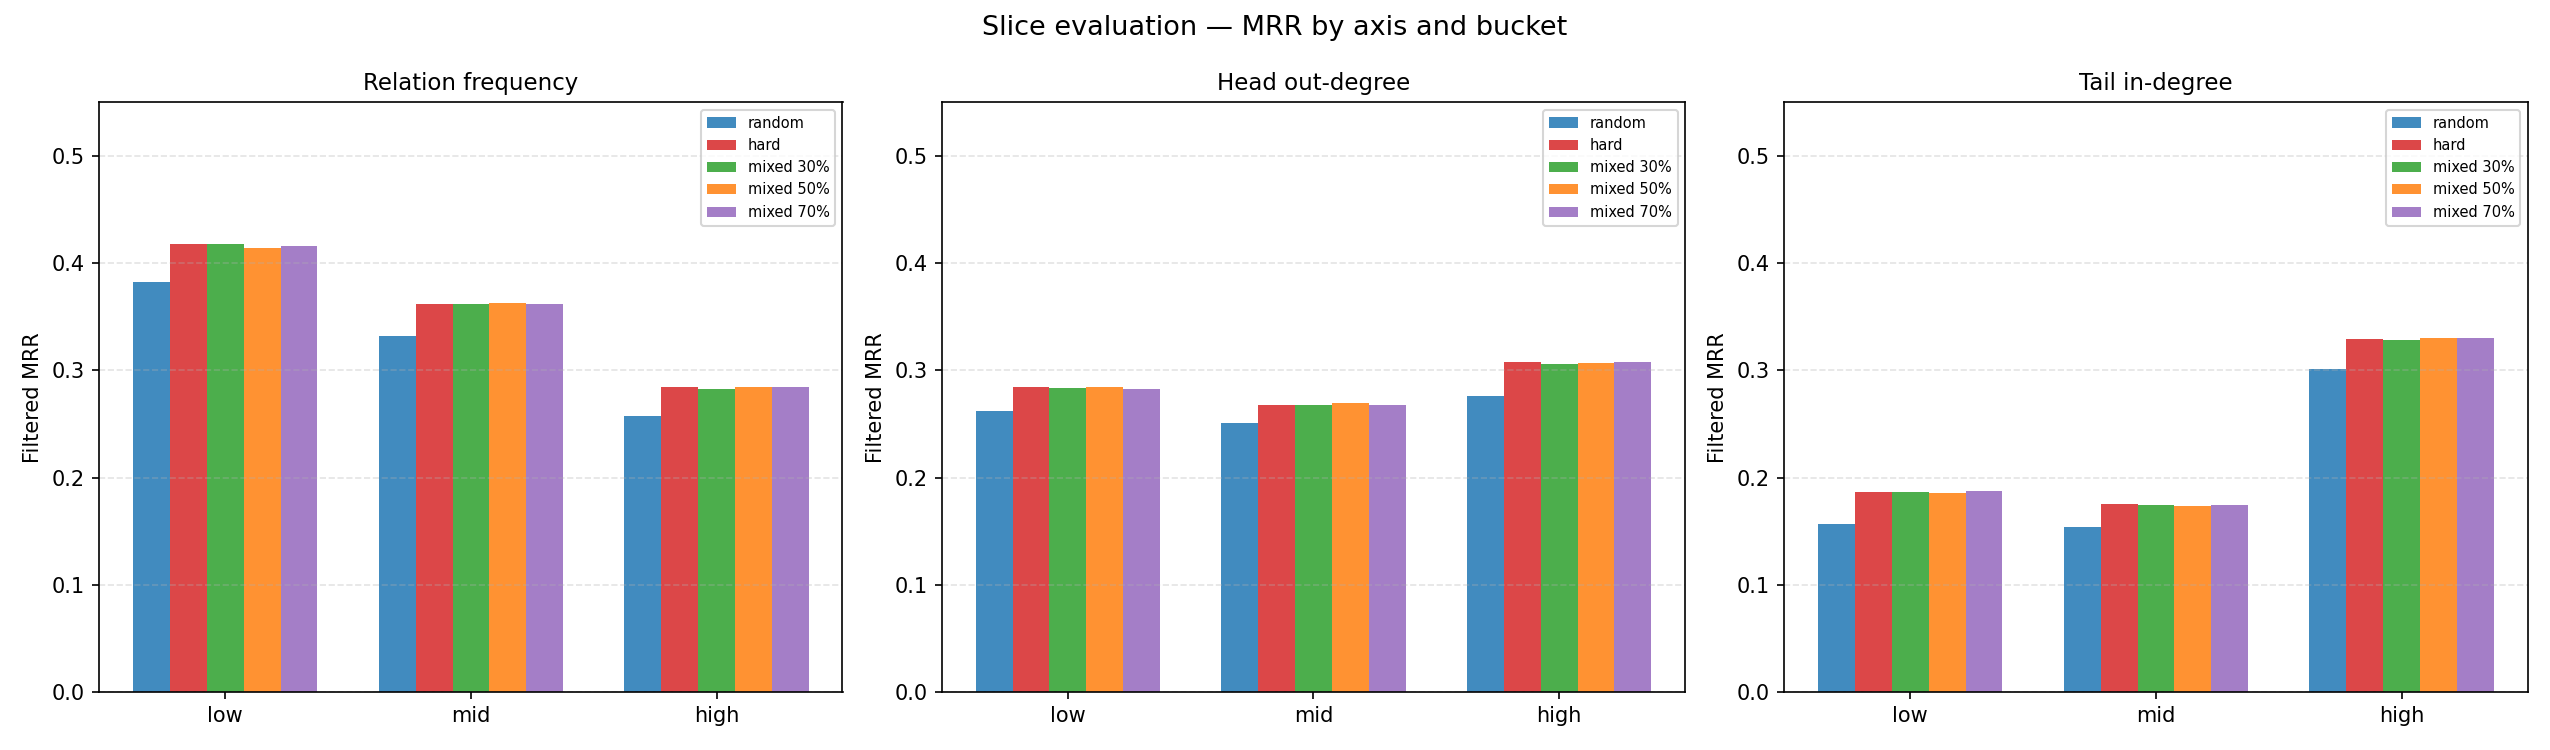
\includegraphics[width=\linewidth]{../../../artifacts/slice_bar_plots.png}
\caption{Slice evaluation: MRR by relation frequency, head out-degree, and tail
in-degree for all five custom strategies. Hard and mixed variants uniformly
dominate the random baseline in every bucket.}
\label{fig:slices}
\end{figure}

%% ────────────────────────────── 7. QUALITATIVE ANALYSIS ─────────────────────
\section{Qualitative Analysis}
\label{sec:qualitative}

We sample five representative test triples and compare the filtered rank of the
correct entity across all five custom strategies. Results are generated by
\texttt{qualitative\_examples.py} using the committed checkpoints (no retraining).

Table~\ref{tab:qualitative} shows two illustrative examples drawn from the
full report. In both cases, hard-negative training substantially reduces the
rank of the correct entity compared to random sampling.

\begin{table}[h]
\centering\scriptsize
\caption{Filtered rank of the gold entity for two representative test
triples, across all five strategies (lower is better).
R1: \emph{tail} prediction for a film regional-release-date relation
(\texttt{release\_date\_s\ldots film\_release\_region}).
R2: \emph{head} prediction for \texttt{/location/location/contains}.
Full paths in \texttt{artifacts/qualitative.md}.}
\label{tab:qualitative}
\begin{tabular}{@{}lcc@{}}
\toprule
Strategy   & R1 (film, tail) & R2 (location, head) \\
\midrule
Random     &  9 & 17 \\
Hard       &  1 &  6 \\
Mixed 30\% &  1 &  4 \\
Mixed 50\% &  3 &  5 \\
Mixed 70\% &  3 &  4 \\
\bottomrule
\end{tabular}
\end{table}

\noindent A recurring pattern is:
\begin{itemize}
  \item For \textbf{structured relations with few valid answers}
    (R1: film release region),
    hard-negative training reduces the rank of the correct entity
    from rank~9 (random) to rank~1.
    Mixed~30\% matches pure hard here, confirming that even a small dose
    of hard negatives is sufficient to learn the tight boundaries of
    this relation type.
  \item For \textbf{high-fanout relations}
    (R2: \texttt{/location/location/contains}),
    tail prediction remains hopeless for all strategies
    (rank~320--1032), as thousands of entities plausibly satisfy the
    query. Head prediction, however, improves consistently: random
    places the correct head at rank~17; hard and all mixed variants
    reach rank~4--6. This asymmetry confirms that hard negatives help
    where the embedding space is dense enough to discriminate.
  \item \textbf{Mixed strategies} match or exceed pure hard on both
    examples (Mixed~30\% achieves rank~1 and rank~4 vs.\ Hard's 1
    and~6), consistent with the aggregate $<\!0.2$~pp MRR gap.
\end{itemize}

\noindent The full qualitative report (5 triples $\times$ 5 strategies, top-10
predictions per query) is committed at \texttt{artifacts/qualitative.md}.

%% ─────────────────────────────── 8. DISCUSSION ──────────────────────────────
\section{Discussion}
\label{sec:discussion}

\paragraph{Hard negatives help, but the gain is bounded.}
The $+10.4\%$ MRR improvement from hard selection is real and consistent, but
all custom runs still score below 0.30 MRR.
The bottleneck is the expressiveness of RotatE itself on 1-to-N and
many-to-many relations, not the sampling strategy.
Relation-specific results confirm this: even the best strategy reaches only
MRR~$\approx0.188$ on low-degree tail entities, where data sparsity is the
fundamental constraint.

\paragraph{30\% hard is the practical sweet spot.}
Mixed~30\% recovers 95\% of the hard-negative gain at no additional compute
cost (all strategies score the same $n=64$ pool). Its lower hard fraction
preserves gradient diversity and keeps training stable at early epochs when
model scores are poorly calibrated. We recommend mixed~30\% as the default
for practitioners working within a fixed compute budget.

\paragraph{Computational cost.}
Timings are approximate (not formally recorded) and were observed on a single
NVIDIA~T4 GPU (Google Colab).
Each of the five custom RotatE runs took $\sim\!1$~hour (50 epochs), for a
total of $\sim\!5$~hours across all strategies.
Baseline training (TransE + RotatE via PyKEEN) took $\sim\!30$~minutes in
total.
Slice evaluation (\texttt{evaluate\_slices.py --all}) required $\sim\!5$~minutes.
The dominant overhead in the custom pipeline is Stage~2, which scores a pool
of $n=64$ candidates per positive triple with the current model before each
gradient step.

\paragraph{Synergy with NSSALoss.}
NSSALoss already performs implicit hard-negative up-weighting via the
adversarial weight $p_i$ (Eq.~\ref{eq:nssa}). Explicit hard selection
concentrates training on the same negatives that receive the largest
$p_i$ weight, producing a doubly amplified gradient signal.
This combination of selection-level and loss-level hard-negative emphasis
is absent when using a uniform-weight loss such as standard margin ranking,
which may contribute to the magnitude of the improvement observed here.

\paragraph{Limitations.}
(1) All experiments use RotatE; the benefit of hard-negative selection on
TransE may differ.
(2) Pool size $n=64$ was not ablated; larger pools may surface harder
negatives and amplify the effect.
(3) Baseline RotatE via PyKEEN and custom RotatE via our pipeline are not
directly comparable in their training infrastructure (different internal
samplers before Stage~2); only the custom runs form a true controlled ablation.

%% ──────────────────────────────── 9. CONCLUSION ──────────────────────────────
\section{Conclusion}
\label{sec:conclusion}

We presented a \textbf{modular two-stage negative sampling pipeline} for
knowledge graph link prediction that decouples filtered pool generation
from strategy-driven selection. A controlled ablation over five strategies
on FB15k-237 shows that:

\begin{enumerate}
  \item \textbf{Hard negatives consistently outperform random sampling}
    ($+0.028$ MRR, $+10.4\%$), confirming that harder gradient signals
    improve embedding quality.
  \item \textbf{30\% hard negatives recover 95\% of the full gain},
    offering an efficient accuracy--compute trade-off.
  \item \textbf{Gains concentrate on rare relations and high-degree entities},
    where the informational value of each gradient step is highest.
  \item \textbf{Head prediction remains systematically harder} than tail
    prediction ($\sim\!0.17$--$0.20$ vs.\ $\sim\!0.37$--$0.40$ MRR),
    a structural property of 1-to-N relations in FB15k-237 that no
    sampling strategy addresses.
\end{enumerate}

The pipeline is orthogonal to model architecture and loss function; future
work could apply it to newer KGE models (e.g.\ RESCAL, TuckER) or combine
it with curriculum scheduling of the hard fraction over training.

%% ──────────────────────────────── INDIVIDUAL CONTRIBUTIONS ──────────────────
\section*{Individual Contributions}

\noindent\textbf{Thalia Delhaise} ---
TODO

\smallskip
\noindent\textbf{Lenny Briclet} ---
TODO

\smallskip
\noindent\textbf{André Fonseca} ---
TODO

\smallskip
\noindent\textbf{Rafael Gufler} ---
TODO

%% ──────────────────────────────── REFERENCES ─────────────────────────────────
{\small
\bibliographystyle{ieeenat_fullname}
\bibliography{../../shared/references}
}

\end{document}
